\hypertarget{RcppExample_8cpp}{
\section{src/RcppExample.cpp File Reference}
\label{RcppExample_8cpp}\index{src/RcppExample.cpp@{src/RcppExample.cpp}}
}
{\tt \#include \char`\"{}Rcpp.h\char`\"{}}\par


Include dependency graph for RcppExample.cpp:\nopagebreak
\begin{figure}[H]
\begin{center}
\leavevmode
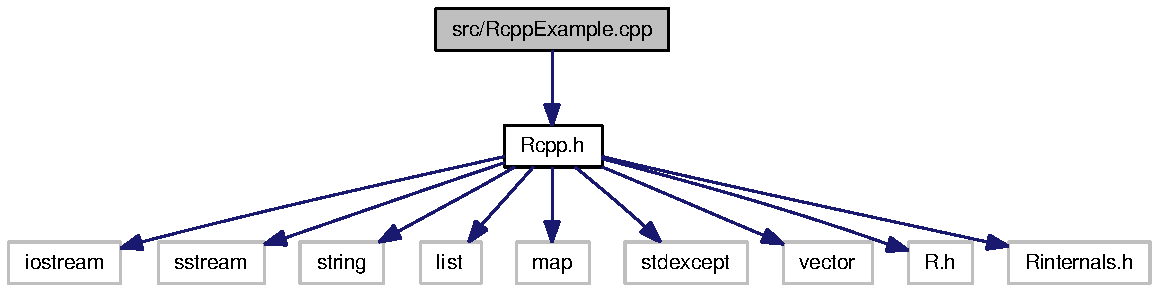
\includegraphics[width=296pt]{RcppExample_8cpp__incl}
\end{center}
\end{figure}
\subsection*{Classes}
\begin{CompactItemize}
\item 
class \hyperlink{classMyRVectorFunc}{MyRVectorFunc}
\item 
class \hyperlink{classMyRListFunc}{MyRListFunc}
\end{CompactItemize}
\subsection*{Functions}
\begin{CompactItemize}
\item 
RcppExport SEXP \hyperlink{RcppExample_8cpp_f892bc38cc3c6c75840941c5d27a316f}{Rcpp\_\-Example} (SEXP params, SEXP nlist, SEXP numvec, SEXP nummat, SEXP df, SEXP datevec, SEXP stringvec, SEXP fnvec, SEXP fnlist)
\item 
RcppExport SEXP \hyperlink{RcppExample_8cpp_44dbfa080dcf3c7ed95e7d0b067276b3}{RcppParamsExample} (SEXP params)
\item 
RcppExport SEXP \hyperlink{RcppExample_8cpp_ecc07b10373d7134c6be02aaa652fc19}{RcppDateExample} (SEXP dvsexp, SEXP dtvsexp)
\item 
RcppExport SEXP \hyperlink{RcppExample_8cpp_4d13d94df70a9a51d67cc6546eb2454f}{RcppVectorExample} (SEXP vector)
\end{CompactItemize}


\subsection{Function Documentation}
\hypertarget{RcppExample_8cpp_f892bc38cc3c6c75840941c5d27a316f}{
\index{RcppExample.cpp@{RcppExample.cpp}!Rcpp\_\-Example@{Rcpp\_\-Example}}
\index{Rcpp\_\-Example@{Rcpp\_\-Example}!RcppExample.cpp@{RcppExample.cpp}}
\subsubsection[{Rcpp\_\-Example}]{\setlength{\rightskip}{0pt plus 5cm}RcppExport SEXP Rcpp\_\-Example (SEXP {\em params}, \/  SEXP {\em nlist}, \/  SEXP {\em numvec}, \/  SEXP {\em nummat}, \/  SEXP {\em df}, \/  SEXP {\em datevec}, \/  SEXP {\em stringvec}, \/  SEXP {\em fnvec}, \/  SEXP {\em fnlist})}}
\label{RcppExample_8cpp_f892bc38cc3c6c75840941c5d27a316f}




Definition at line 109 of file RcppExample.cpp.

References RcppResultSet::add(), MyRListFunc::addOne(), RcppFrame::addRow(), RcppMatrix$<$ T $>$::cMatrix(), copyMessageToR(), RcppVector$<$ T $>$::cVector(), RcppParams::getDateValue(), RcppDate::getDay(), RcppMatrix$<$ T $>$::getDim1(), RcppMatrix$<$ T $>$::getDim2(), RcppParams::getDoubleValue(), RcppParams::getIntValue(), RcppDate::getMonth(), RcppNumList::getName(), RcppResultSet::getReturnList(), RcppParams::getStringValue(), MyRVectorFunc::getSum(), RcppNumList::getValue(), RcppDate::getYear(), RcppVector$<$ T $>$::size(), RcppMatrix$<$ T $>$::stlMatrix(), and RcppVector$<$ T $>$::stlVector().

Here is the call graph for this function:\nopagebreak
\begin{figure}[H]
\begin{center}
\leavevmode
\includegraphics[width=259pt]{RcppExample_8cpp_f892bc38cc3c6c75840941c5d27a316f_cgraph}
\end{center}
\end{figure}
\hypertarget{RcppExample_8cpp_ecc07b10373d7134c6be02aaa652fc19}{
\index{RcppExample.cpp@{RcppExample.cpp}!RcppDateExample@{RcppDateExample}}
\index{RcppDateExample@{RcppDateExample}!RcppExample.cpp@{RcppExample.cpp}}
\subsubsection[{RcppDateExample}]{\setlength{\rightskip}{0pt plus 5cm}RcppExport SEXP RcppDateExample (SEXP {\em dvsexp}, \/  SEXP {\em dtvsexp})}}
\label{RcppExample_8cpp_ecc07b10373d7134c6be02aaa652fc19}




Definition at line 382 of file RcppExample.cpp.

References RcppResultSet::add(), copyMessageToR(), RcppResultSet::getReturnList(), RcppDatetimeVector::size(), and RcppDateVector::size().

Here is the call graph for this function:\nopagebreak
\begin{figure}[H]
\begin{center}
\leavevmode
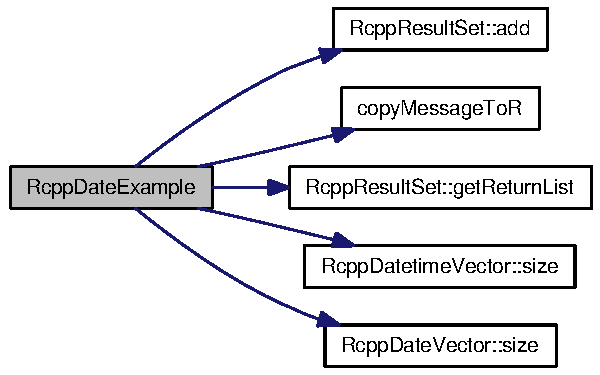
\includegraphics[width=162pt]{RcppExample_8cpp_ecc07b10373d7134c6be02aaa652fc19_cgraph}
\end{center}
\end{figure}
\hypertarget{RcppExample_8cpp_44dbfa080dcf3c7ed95e7d0b067276b3}{
\index{RcppExample.cpp@{RcppExample.cpp}!RcppParamsExample@{RcppParamsExample}}
\index{RcppParamsExample@{RcppParamsExample}!RcppExample.cpp@{RcppExample.cpp}}
\subsubsection[{RcppParamsExample}]{\setlength{\rightskip}{0pt plus 5cm}RcppExport SEXP RcppParamsExample (SEXP {\em params})}}
\label{RcppExample_8cpp_44dbfa080dcf3c7ed95e7d0b067276b3}




Definition at line 333 of file RcppExample.cpp.

References copyMessageToR(), RcppParams::getDateValue(), RcppDate::getDay(), RcppParams::getDoubleValue(), RcppParams::getIntValue(), RcppDate::getMonth(), RcppParams::getStringValue(), and RcppDate::getYear().

Here is the call graph for this function:\nopagebreak
\begin{figure}[H]
\begin{center}
\leavevmode
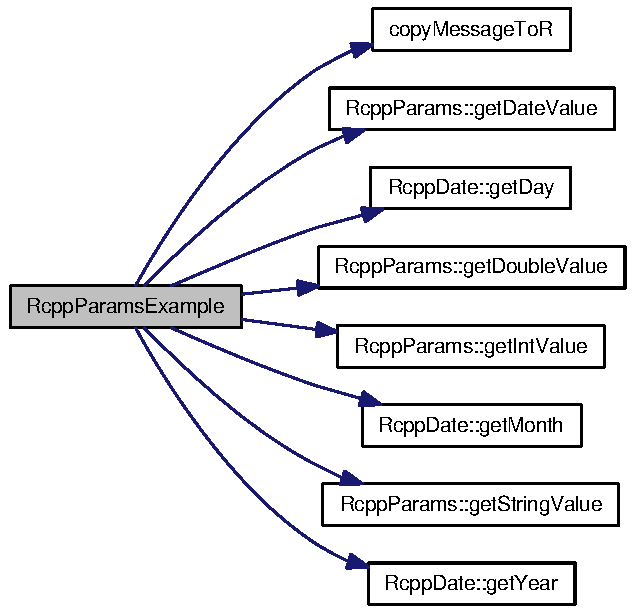
\includegraphics[width=169pt]{RcppExample_8cpp_44dbfa080dcf3c7ed95e7d0b067276b3_cgraph}
\end{center}
\end{figure}
\hypertarget{RcppExample_8cpp_4d13d94df70a9a51d67cc6546eb2454f}{
\index{RcppExample.cpp@{RcppExample.cpp}!RcppVectorExample@{RcppVectorExample}}
\index{RcppVectorExample@{RcppVectorExample}!RcppExample.cpp@{RcppExample.cpp}}
\subsubsection[{RcppVectorExample}]{\setlength{\rightskip}{0pt plus 5cm}RcppExport SEXP RcppVectorExample (SEXP {\em vector})}}
\label{RcppExample_8cpp_4d13d94df70a9a51d67cc6546eb2454f}




Definition at line 423 of file RcppExample.cpp.

References RcppResultSet::add(), copyMessageToR(), RcppResultSet::getReturnList(), and RcppVector$<$ T $>$::size().

Here is the call graph for this function:\nopagebreak
\begin{figure}[H]
\begin{center}
\leavevmode
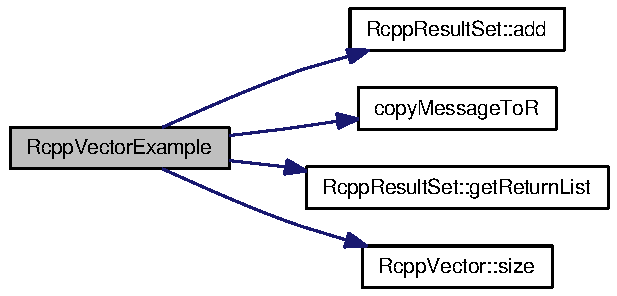
\includegraphics[width=166pt]{RcppExample_8cpp_4d13d94df70a9a51d67cc6546eb2454f_cgraph}
\end{center}
\end{figure}
